% =============================================================================
% Lecture 04: Decision Trees
% ECON 8310: Business Forecasting
% University of Nebraska at Omaha
% =============================================================================

\documentclass[aspectratio=169, 11pt]{beamer}

\input{header}

% ---- Lecture metadata --------------------------------------------------------
\title[Decision Trees]{Decision Trees}
\subtitle{ECON 8310: Business Forecasting --- Lecture 4}
\author{Department of Economics}
\institute{University of Nebraska at Omaha}

% =============================================================================
\begin{document}
% =============================================================================

\begin{frame}
  \titlepage
\end{frame}

% ---- Outline ----------------------------------------------------------------
\begin{frame}{Lecture Outline}
  \tableofcontents
\end{frame}

% =============================================================================
\section{Why Go Beyond Linear Models?}
% =============================================================================

\sectionslide{Why Go Beyond Linear Models?}{%
  Real-world relationships are often nonlinear, involve interactions,
  and shift with context.}

% --- Slide: Linear model limitation ------------------------------------------
\begin{frame}{The Limits of Linear Models}
  \textbf{Three things a constant slope cannot represent:}
  \begin{itemize}
    \item \textbf{Interactions} --- the holiday-season advertising effect
          is not a constant slope
    \item \textbf{Threshold effects} --- spending may be flat until
          unemployment drops below 5\%, then jump
    \item \textbf{Asymmetry} --- a rise and a fall of the same size move the
          forecast equally, even when the real response is lopsided
  \end{itemize}
  \begin{examplebox}{Retail Sales Example}
    Monthly sales depend on last year's same-month sales (trend),
    whether it is December (seasonality), and the unemployment rate
    (conditions). The December effect is \emph{larger} in a strong
    economy --- an interaction a linear model misses.
  \end{examplebox}
  \textbf{Decision trees capture nonlinearity and interactions automatically},
  without your having to specify them in advance.
\end{frame}

% --- Slide: Bias-variance tradeoff overview ----------------------------------
% Figure: scripts/figures/lecture04_figures.py (stumps_vs_deep); numbers in measured.json
% ("bootstrap"). One test week, chosen as an illustration; the 52-week averages agree.
\begin{frame}{The Bias--Variance Tradeoff \parencite{James2021}}
  \begin{definitionbox}{Bias--Variance Decomposition}
    \[
      \text{Expected MSE} = \underbrace{\text{Bias}^2}_{\text{systematic error}}
                           + \underbrace{\text{Variance}}_{\text{sensitivity to data}}
                           + \underbrace{\sigma^2}_{\text{irreducible noise}}
    \]
  \end{definitionbox}
  \vspace{-0.3cm}
  \begin{center}
    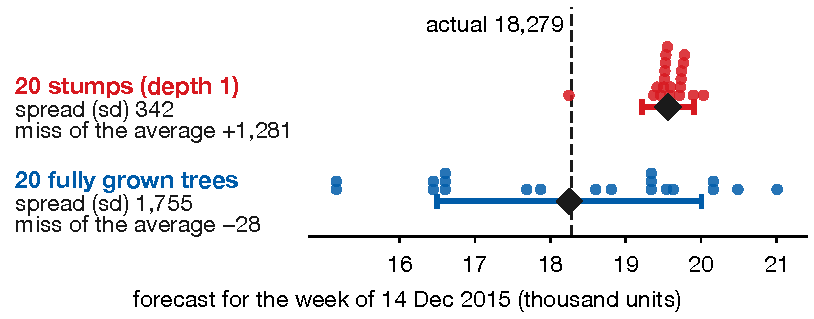
\includegraphics[height=3.3cm]{../Figures/Lecture04_DecisionTrees/stumps_vs_deep.pdf}
  \end{center}
  \vspace{-0.4cm}
  {\small Weekly CA\_1 FOODS, 20 bootstrap refits per model. \textbf{Stumps} (one-question trees)
  agree and miss: bias. \textbf{Deep trees} center on the truth but scatter: variance. (The miss
  includes noise, so it is not pure bias.) \textbf{Goal:} the complexity that
  balances the two, visible only \emph{out-of-sample}.}
\end{frame}

% =============================================================================
\section{How Decision Trees Work}
% =============================================================================

\sectionslide{How Decision Trees Work}{%
  Partition the feature space into rectangles; predict the mean in each region.}

% --- Slide: The tree metaphor ------------------------------------------------
% The real depth-2 tree on weekly CA_1 FOODS (173 training weeks); every number is in
% Figures/Lecture04_DecisionTrees/measured.json ("depth2"), written by
% scripts/figures/lecture04_figures.py. Thresholds x.5 on integer units are printed as <= x.
% Coordinates (x, y), cm:
%   root (4.9, 0)        -- y_{t-4} <= 20,603?
%   L1   (2.1, -1.25)    -- y_{t-4} <= 18,598?      R1 (7.7, -1.25) -- y_{t-52} <= 21,692?
%   leaves at y = -2.55: (0.7), (3.5), (6.3), (9.1) -- 18,399 / 20,110 / 21,434 / 22,988
\begin{frame}{What Is a Decision Tree?}
  A flowchart of yes/no questions about the features, ending in a prediction. Here is the real
  depth-2 tree for weekly CA\_1 FOODS units:

  \vspace{0.05cm}
  \begin{center}
    \begin{tikzpicture}[
      every node/.style={font=\small},
      internal/.style={rectangle, rounded corners=3pt,
        fill=unolightcrimson, draw=unocrimson, line width=0.8pt,
        align=center, inner sep=3pt, text width=3.2cm,
        minimum width=3.4cm, minimum height=0.6cm},
      leaf/.style={rectangle, rounded corners=3pt,
        fill=unolightgreen, draw=unogreen, line width=0.8pt,
        align=center, inner sep=3pt, text width=2.2cm,
        minimum width=2.4cm, minimum height=0.85cm},
    ]
      \node[internal] (root) at (4.9, 0)     {$y_{t-4} \leq 20{,}603$?};
      \node[internal] (l1)   at (2.1, -1.25) {$y_{t-4} \leq 18{,}598$?};
      \node[internal] (r1)   at (7.7, -1.25) {$y_{t-52} \leq 21{,}692$?};
      \node[leaf] (a) at (0.7, -2.55) {$\hat{y} = 18{,}399$\\[-1pt]{\scriptsize 27 weeks}};
      \node[leaf] (b) at (3.5, -2.55) {$\hat{y} = 20{,}110$\\[-1pt]{\scriptsize 62 weeks}};
      \node[leaf] (c) at (6.3, -2.55) {$\hat{y} = 21{,}434$\\[-1pt]{\scriptsize 59 weeks}};
      \node[leaf] (d) at (9.1, -2.55) {$\hat{y} = 22{,}988$\\[-1pt]{\scriptsize 25 weeks}};
      \draw[->, gray] (root) -- (l1) node[midway, above left, font=\tiny]{Yes};
      \draw[->, gray] (root) -- (r1) node[midway, above right, font=\tiny]{No};
      \draw[->, gray] (l1) -- (a) node[midway, left, font=\tiny]{Yes};
      \draw[->, gray] (l1) -- (b) node[midway, right, font=\tiny]{No};
      \draw[->, gray] (r1) -- (c) node[midway, left, font=\tiny]{Yes};
      \draw[->, gray] (r1) -- (d) node[midway, right, font=\tiny]{No};
    \end{tikzpicture}
  \end{center}
  \vspace{-0.15cm}
  {\small \textbf{Non-parametric} $\cdot$ \textbf{nonlinear} (captures thresholds) $\cdot$
  \textbf{interpretable} $\cdot$ \textbf{scale-invariant}. A single \emph{deep} tree
  \textbf{overfits severely}; ensembles, the next lecture, are the fix.}

  \muted{\footnotesize $y_{t-4}$: units four weeks earlier; $y_{t-52}$: the same week last year.
  Fitted on the 173 weeks before the test year.}
\end{frame}

% --- Slide: the tree as rectangles -------------------------------------------
% Figure: scripts/figures/lecture04_figures.py (tree_partition): the depth-2 tree above, drawn in
% the plane of the two features it uses; cuts and leaf means read from measured.json ("depth2").
\begin{frame}{The Same Tree, Drawn as Rectangles}
  Each question is a straight cut parallel to an axis. Each leaf is a rectangle, shaded by its
  mean; every week inside it gets that forecast.
  \begin{center}
    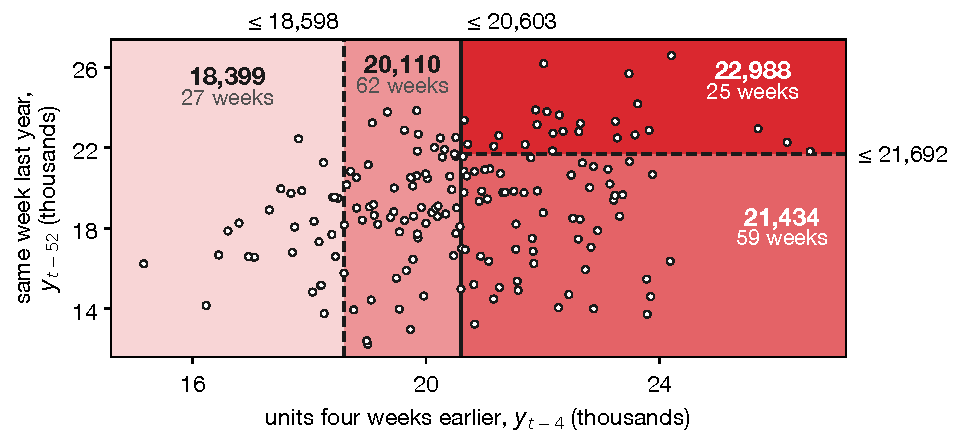
\includegraphics[height=4.75cm]{../Figures/Lecture04_DecisionTrees/tree_partition.pdf}
  \end{center}
  \vspace{-0.3cm}
  {\small Last year's sales cut only the right half: they matter only when recent demand is
  already high. That is an \textbf{interaction}, and nobody specified it.}
\end{frame}

% --- Slide: CART algorithm ---------------------------------------------------
% Figure: scripts/figures/lecture04_figures.py cart_split (numbers in measured.json, "root").
\begin{frame}{The CART Algorithm (Regression) \parencite{Breiman1984}}
  \begin{columns}[T]
    \begin{column}{0.42\textwidth}
      At each node, CART tries every feature $j$ and threshold $t$, and keeps the split with the
      least squared error:
      {\small
      \[
        \textstyle\sum_{x_{ij} \leq t} (y_i - \bar{y}_{L})^2 + \sum_{x_{ij} > t} (y_i - \bar{y}_{R})^2
      \]}%
      Each leaf predicts its mean; then repeat inside each group.

      \vspace{0.15cm}
      \textbf{Geometrically:} slide the cut and total the squared vertical sticks. Our best first
      cut, $y_{t-4} \leq 20{,}603$, removes 35\% of the squared error.

      \vspace{0.1cm}
      \muted{\footnotesize Classification uses Gini impurity or entropy instead.}
    \end{column}
    \begin{column}{0.56\textwidth}
      \centering
      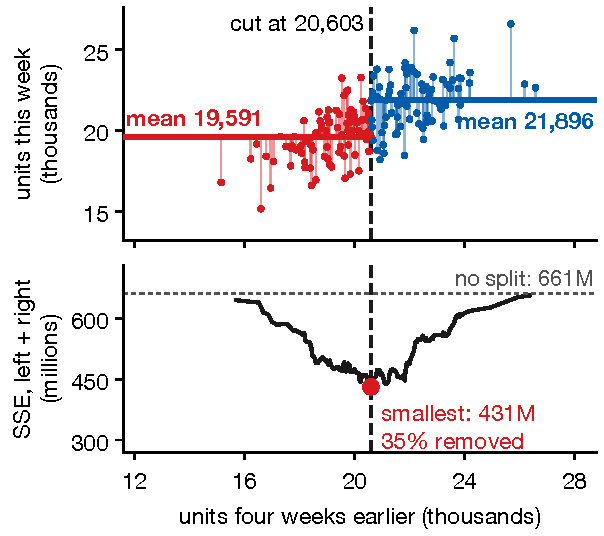
\includegraphics[height=5.9cm]{../Figures/Lecture04_DecisionTrees/cart_split.pdf}
    \end{column}
  \end{columns}
\end{frame}

% --- Slide: greedy is not optimal --------------------------------------------
\begin{frame}{Greedy Is Not Optimal --- and That Matters}
  CART is \textbf{exhaustive} at each node: it tries every feature and every threshold. But it
  is \textbf{greedy} across nodes: it never looks ahead. An illustration:
  \begin{center}
    {\small
    \begin{tabular}{lcc}
      \toprule
      \textbf{Split at the root} & \textbf{Variance removed now} & \textbf{\ldots plus what it enables} \\
      \midrule
      On price     & \textbf{40\%} & $+$ 12\% \quad (total 52\%) \\
      On promotion & 38\%          & $+$ 50\% \quad \textbf{(total 88\%)} \\
      \bottomrule
    \end{tabular}
    }
  \end{center}
  \vspace{-0.1cm}
  CART takes the 40\%. It cannot see the 50\% coming: it scores one split at a time.

  \vspace{0.15cm}
  So a fitted tree is a sequence of locally best choices, \textbf{not the optimal tree} (finding
  that is intractable). It can \textbf{miss real structure}, and a small change in the data can
  send the greedy sequence down a different path: the instability we turn to next.
\end{frame}

% --- Slide: Bias-variance in trees -------------------------------------------
% Figure: scripts/figures/lecture04_figures.py (depth_curve); numbers in measured.json ("depth_sweep").
\begin{frame}{Depth Controls the Bias--Variance Tradeoff}
  A \textbf{stump} asks one question: high bias, low variance. A \textbf{full tree}, one week per
  leaf, memorizes the sample: zero \emph{training} error, high variance.
  \begin{center}
    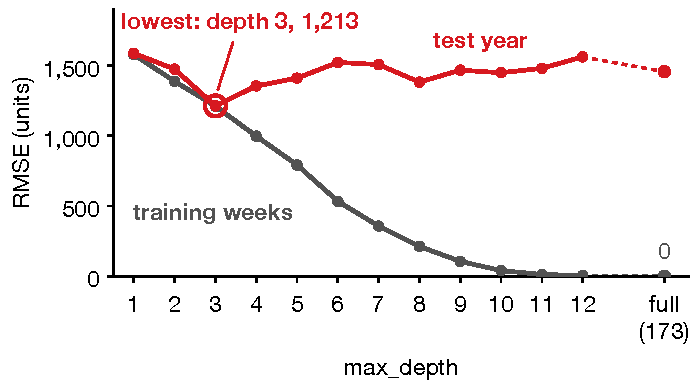
\includegraphics[height=4.1cm]{../Figures/Lecture04_DecisionTrees/depth_curve.pdf}
  \end{center}
  \vspace{-0.35cm}
  {\small Weekly CA\_1 FOODS, one week ahead (seasonal naive: 1,660). Training error falls to
  zero; test error stops improving after depth 3 (only 173 weeks). Read
  the shape, not the minimum: picking depth from the test year is a leak. \textbf{Unstable,
  too:} one changed week can flip the root split, and everything below it. Tune by
  \texttt{TimeSeriesSplit}.}
\end{frame}

% --- Slide: pruning ----------------------------------------------------------
\begin{frame}{Two Ways to Stop a Tree Overfitting}
  \texttt{max\_depth} caps the tree in advance. Two other controls do the job better.
  \begin{center}
    {\small
    \begin{tabular}{p{3.2cm}p{9.2cm}}
      \toprule
      \texttt{min\_samples\_leaf} & \textbf{Stop early.} At the default of 1, a leaf may hold a
      single observation and ``predict'' that one value. Set it to 5--10 and every prediction is
      an average over a real group. \\[3pt]
      \texttt{ccp\_alpha} & \textbf{Prune after.} Grow the tree out fully, then charge a penalty
      $\alpha$ per leaf and cut back the branches that do not pay for themselves. \\
      \bottomrule
    \end{tabular}
    }
  \end{center}
  Choose either one by \texttt{TimeSeriesSplit} cross-validation, never by the test year.
\end{frame}

% --- Slide: pruning, drawn ---------------------------------------------------
% Figure: scripts/figures/lecture04_figures.py pruning_hull (numbers in measured.json, "pruning").
\begin{frame}{Cost-Complexity Pruning: A Line Touching the Curve}
  Pruning minimizes $\sum_{\text{leaves}} \text{SSE} + \alpha\,|T|$: the fit, plus a price
  $\alpha$ for each of the $|T|$ leaves. Each black dot is the best pruned tree for some range of
  $\alpha$.
  \begin{center}
    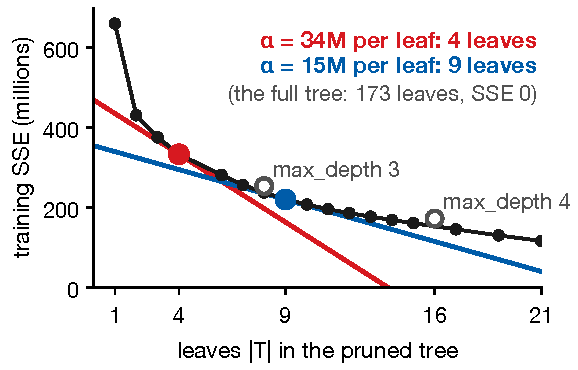
\includegraphics[height=4.15cm]{../Figures/Lecture04_DecisionTrees/pruning_hull.pdf}
  \end{center}
  \vspace{-0.3cm}
  {\small Push a line of slope $-\alpha$ up from below: the first dot it touches is the tree
  $\alpha$ picks. A bigger $\alpha$ tilts it and picks a smaller tree. The 4-leaf tree is the
  flowchart from earlier.}

  \muted{\footnotesize The same idea as Lecture 3's smoothing penalty and Lecture 6's Ridge and
  LASSO; $\alpha$ is chosen by cross-validation. scikit-learn's \texttt{ccp\_alpha} is
  $\alpha/n$.}
\end{frame}

% =============================================================================
\section{Implementing Decision Trees in Python}
% =============================================================================

\sectionslide{Implementing Decision Trees in Python}{%
  One class, a few hyperparameters, interpretable results.}

% --- Slide: sklearn implementation -------------------------------------------
\begin{frame}{Decision Tree Regression in Python}
  \begin{examplebox}{sklearn Code Template}
    {\scriptsize
    \texttt{from sklearn.tree import DecisionTreeRegressor}\\
    \texttt{X, y = weekly[FEATURES], weekly['units']\ \ \# lags, SNAP, events, price}\\
    \texttt{tree = DecisionTreeRegressor(max\_depth=5, min\_samples\_leaf=10, random\_state=42)}\\
    \texttt{tree.fit(X\_train, y\_train);\ \ y\_hat = tree.predict(X\_test)}
    }
  \end{examplebox}
  \vspace{-0.15cm}
  \begin{center}
    {\footnotesize
    \begin{tabular}{ll}
      \toprule
      \textbf{Parameter} & \textbf{Effect} \\
      \midrule
      \texttt{max\_depth}         & Cap tree depth \\
      \texttt{min\_samples\_leaf} & Minimum observations per leaf \\
      \texttt{max\_features}      & Feature subsampling \\
      \texttt{ccp\_alpha}         & Cost-complexity pruning \\
      \bottomrule
    \end{tabular}
    }
  \end{center}
  \vspace{-0.15cm}
  {\small Cross-validate with \texttt{TimeSeriesSplit}, never \texttt{KFold} ---
  \textbf{random folds leak the future into the training set}.}
\end{frame}

% --- Slide: Feature importance -----------------------------------------------
\begin{frame}{Feature Importance \parencite{Molnar2022}}
  \begin{definitionbox}{Impurity-Based Feature Importance}
    For each feature $j$, sum the total reduction in variance across all splits
    where $j$ was used, weighted by the fraction of observations in each node.
    Normalize so the importances sum to 1.
  \end{definitionbox}
  \begin{center}
    {\small
    \begin{tabular}{lc}
      \toprule
      \textbf{Feature (CA\_1 FOODS, weekly)} & \textbf{Importance} \\
      \midrule
      \texttt{units\_lag4}  & 0.62 \\
      \texttt{units\_lag52} & 0.15 \\
      \texttt{units\_lag1}  & 0.13 \\
      \texttt{snap\_days}   & 0.05 \\
      \texttt{avg\_price}   & 0.04 \\
      \bottomrule
    \end{tabular}
    }
  \end{center}
  \vspace{-0.1cm}
  From the previous slide's depth-5 tree. Read it as a list of what the tree leaned on: a fast
  way to screen predictors.
  \muted{\footnotesize But impurity importance is biased toward
  features with many split points. Permutation importance gives a more
  reliable ranking; we return to it in Lecture 5.}
\end{frame}

% --- Slide: Interpreting tree predictions ------------------------------------
\begin{frame}{Interpreting and Communicating Tree Predictions}
  A tree's main advantage is that you can explain \emph{why} a specific
  prediction was made.
  \begin{examplebox}{Explaining a Prediction to a Manager}
    ``Our model forecasts 22,988 units for this week because:
    \begin{enumerate}\small
      \item Four weeks ago the store sold more than 20,603 units (recent demand is high)
      \item The same week last year sold more than 21,692 (the season is strong)
      \item The 25 training weeks where both held averaged 22,988 units.''
    \end{enumerate}
  \end{examplebox}
  Produce the path with \texttt{sklearn.tree.plot\_tree(tree)} or
  \texttt{export\_text(tree, feature\_names=[...])}.
  \muted{\footnotesize This is where business buy-in comes from --- a manager
  can check that the tree is splitting on variables they consider sensible.}
\end{frame}

% =============================================================================
\section{Limitations and Preview: Ensembles}
% =============================================================================

\sectionslide{Limitations and Preview: Ensembles}{%
  A single tree is a weak learner. Combine hundreds to build a strong one.}

% --- Slide: When trees fail ---------------------------------------------------
\begin{frame}{When a Single Tree Falls Short}
  \begin{columns}[T]
    \begin{column}{0.48\textwidth}
      \textbf{Strengths:}
      {\setbeamertemplate{itemize item}{\pos{$\checkmark$}}
      \begin{itemize}\small
        \item Interpretable --- can show the path
        \item No feature scaling needed
        \item Captures nonlinear relationships
        \item Handles missing values well
        \item Fast to train
      \end{itemize}}
    \end{column}
    \begin{column}{0.48\textwidth}
      \textbf{Weaknesses:}
      {\setbeamertemplate{itemize item}{\negc{$\times$}}
      \begin{itemize}\small
        \item High variance --- small data changes give a very different tree
        \item Flat predictions within each leaf
        \item Cannot extrapolate beyond the training range
        \item Sensitive to outliers in a leaf
      \end{itemize}}
    \end{column}
  \end{columns}
  \vspace{0.2cm}
  \textbf{The ensemble solution:} average many trees fitted to bootstrap samples. Variance falls
  sharply and feature importance survives, typically for 20--40\% lower RMSE than one tree.
\end{frame}

% --- Slide: Key takeaways ---------------------------------------------------
\begin{frame}{Lecture 4: Key Takeaways}
  \begin{keybox}
    {\small
    \begin{enumerate}
      \item Trees capture \textbf{interactions} and \textbf{thresholds} without being told.
      \item Depth sets the \textbf{bias--variance} tradeoff: too shallow underfits, too deep
            overfits.
      \item \textbf{CART} takes the split with the least squared error; a leaf predicts its mean.
      \item Stop overfitting with \texttt{min\_samples\_leaf} or \texttt{ccp\_alpha}, tuned by
            \texttt{TimeSeriesSplit}.
      \item Trees are \textbf{interpretable}: you can read the path to any prediction.
      \item A tree is a \textbf{step function} that cannot extrapolate; its \textbf{high
            variance} needs ensembles (Lecture 5).
    \end{enumerate}
    }
  \end{keybox}
  \muted{\itshape Next: Tree Ensembles --- variance reduction through
  bootstrap aggregation, and sequential error correction with boosting.}
\end{frame}

% --- References ---------------------------------------------------------------
\begin{frame}[allowframebreaks]{References}
  \printbibliography[heading=none]
\end{frame}

% =============================================================================
\end{document}
% =============================================================================
